\section{Task 3 - LID-Augmented MuRIL}

Adding the language tags gives a test macro-F1 of 0.598. That's above Task 1 (0.583) but slightly below plain MuRIL (0.606).

\subsection*{Implementation}
\textbf{Implemented option:} a learned tag embedding for every subword (not the summary token).
\begin{enumerate}
    \item Each word has the tag the Task 1 LID tagger predicted for it, and every subword of that word inherits it. \texttt{[CLS]}, \texttt{[SEP]} and padding get a fourth tag, \texttt{special}.
    \item A learned 16-dim tag embedding is concatenated to MuRIL's 768-dim word embedding, giving 784 dims.
    \item MuRIL's layers expect 768 dims, so the 784 are mapped back with the matrix $[\mathbf{I} \mid \mathbf{W\_tag}]$. The identity on the word part stays fixed, and only $\mathbf{W\_tag}$ ($768 \times 16$) is learned, starting at zero. Training therefore starts exactly from plain MuRIL.
    \item The result goes into MuRIL as \texttt{inputs\_embeds}, before the transformer layers. The input is the Dakshina-normalized text, and every hyperparameter is the same as in Task 2.
\end{enumerate}



\begin{figure}[H]
    \centering
    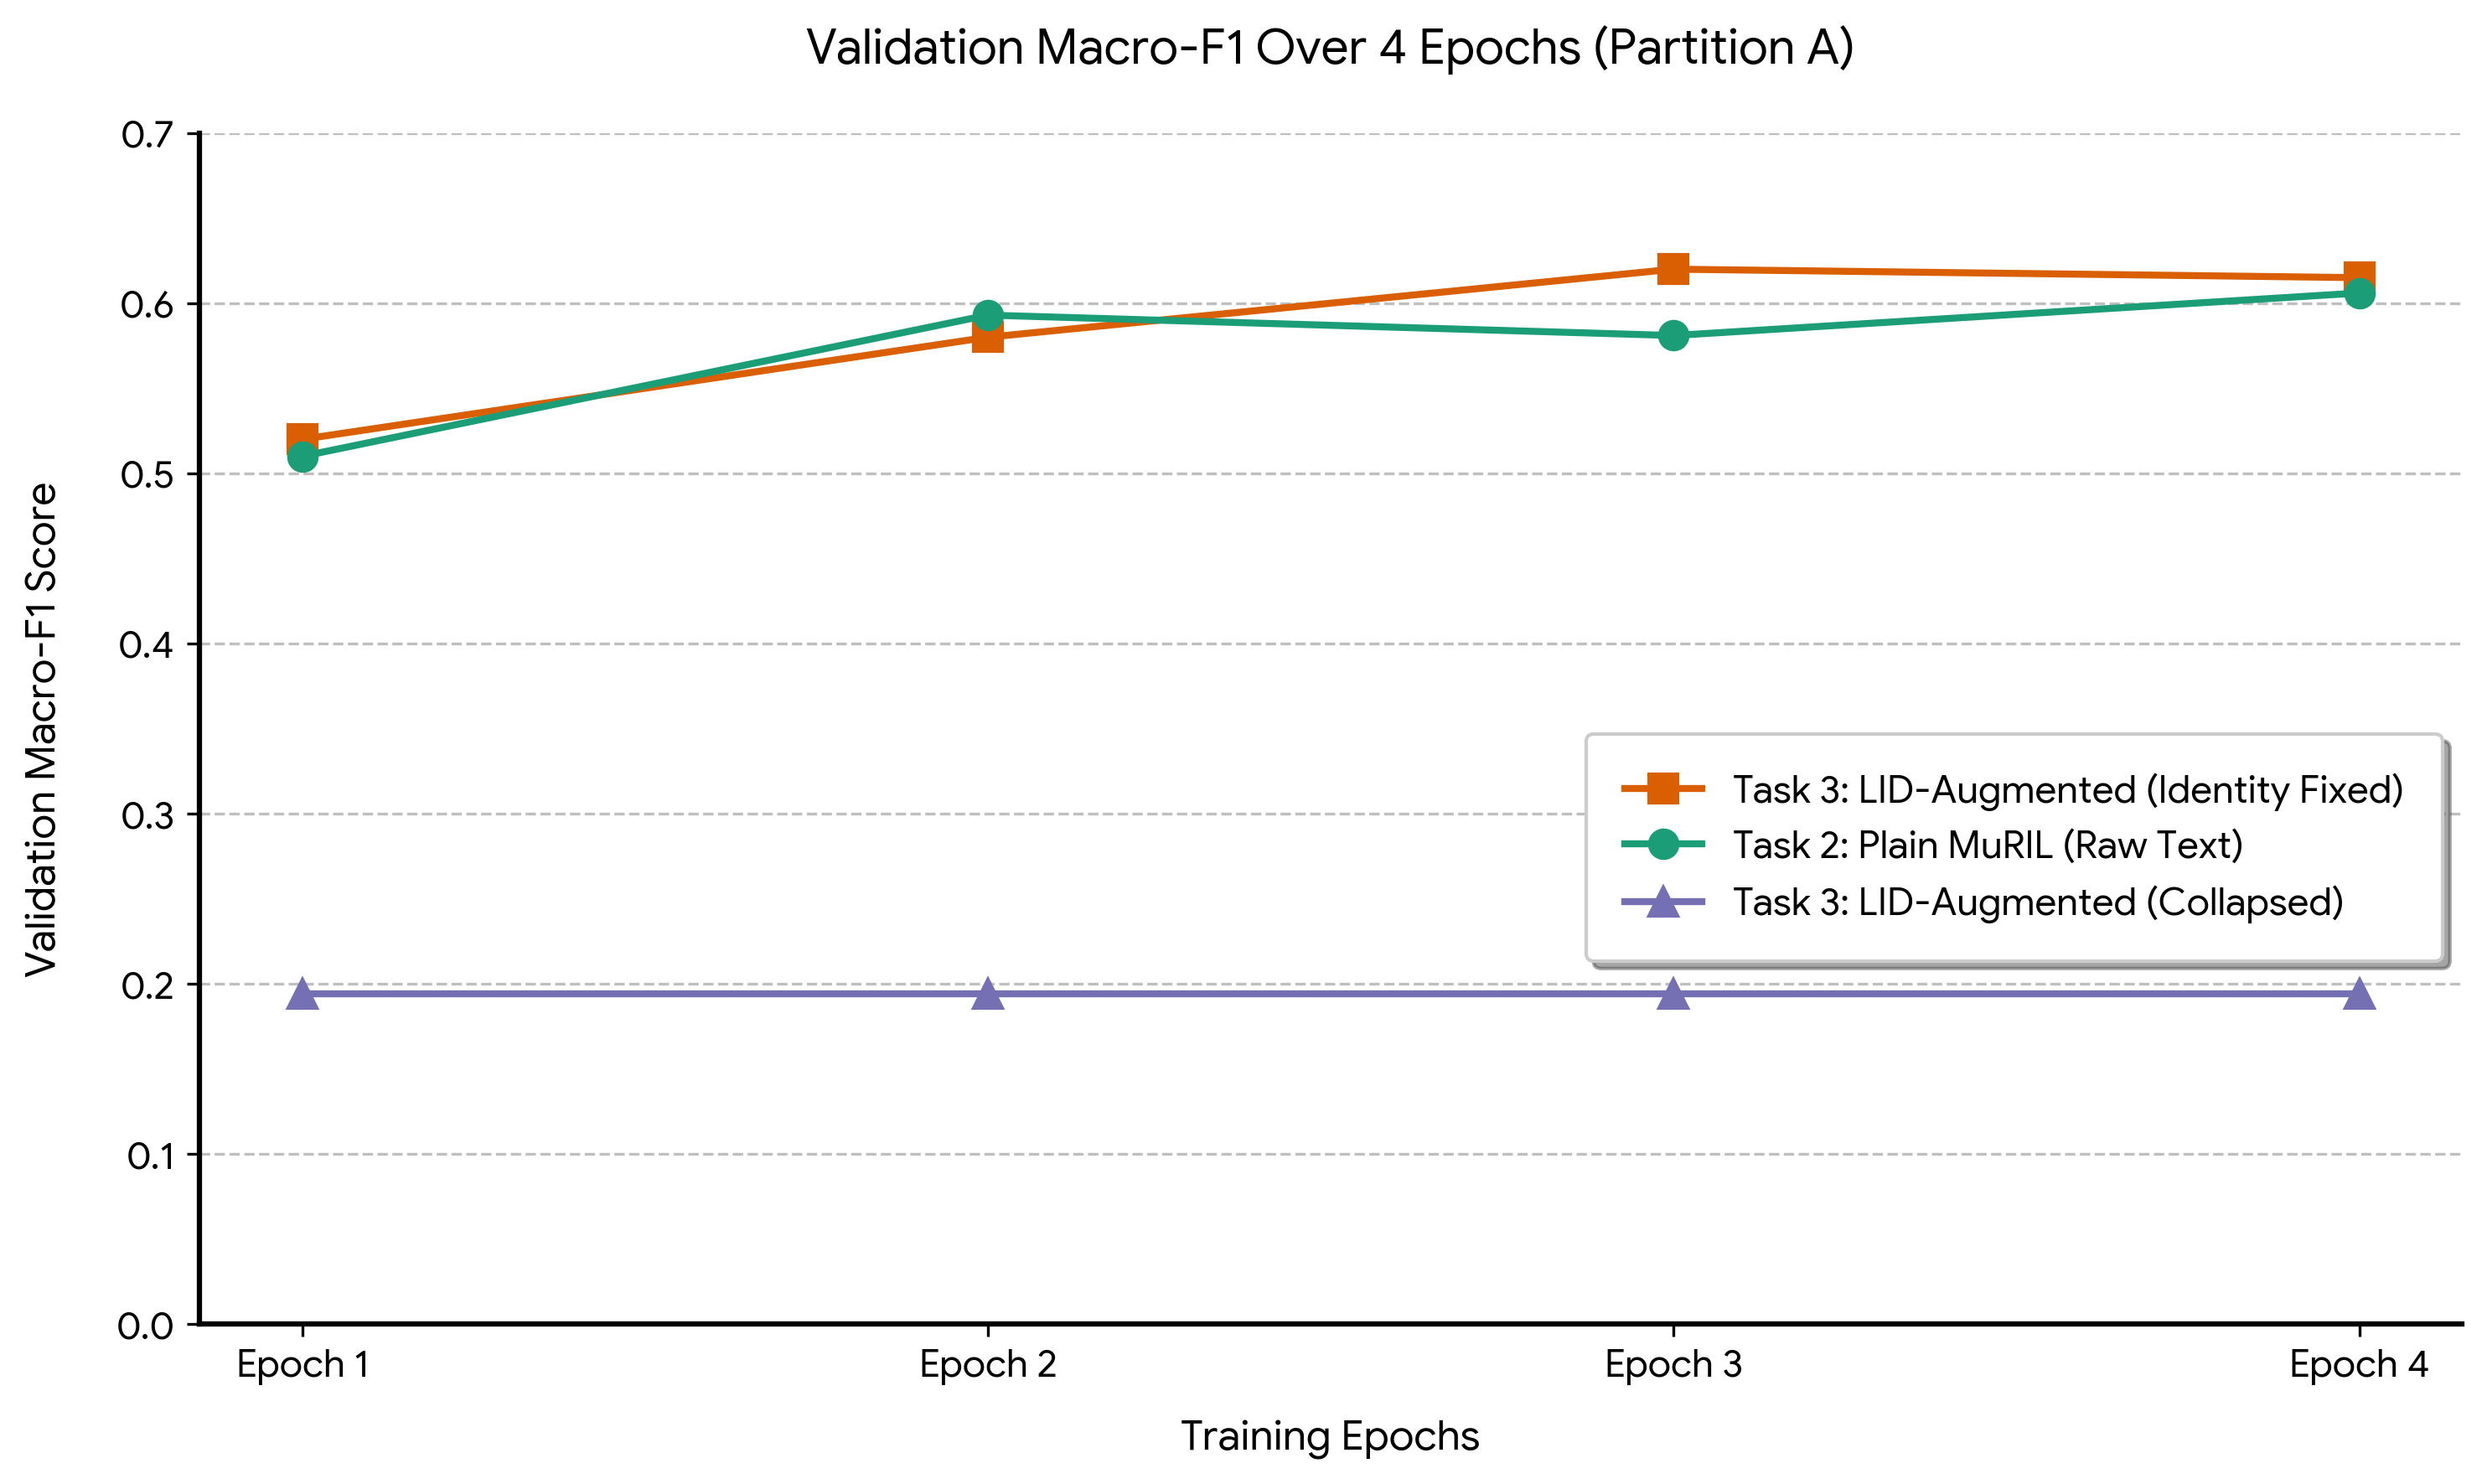
\includegraphics[width=0.95\textwidth]{task3_validation_curve_new.png}
    \caption{Validation Macro-F1 across 4 epochs on the Partition A validation split. Fixing the identity matrix allowed the LID-augmented model to converge successfully.}
    \label{fig:val_f1_curve}
\end{figure}

\textbf{The first version collapsed.} It learned the whole $784 \rightarrow 768$ matrix, starting from the identity. AdamW moves each of its $\sim$590,000 weights by about the learning rate at every step, so MuRIL's word embeddings drifted by about 10\% in a 150-step test. The model then predicted ``neutral'' for every tweet (test macro-F1 0.194). Keeping the identity fixed solved it.

\subsection*{Results and Discussion}

\textbf{Quantitative Results:} \\
After 4 epochs of fine-tuning using our custom PyTorch training loop, the LID-augmented MuRIL model achieved a macro-F1 score of 0.598 on the Partition A test split. 

\begin{table}[H]
    \centering
    \begin{tabular}{@{}ll@{}}
        \toprule
        \textbf{Model Configuration} & \textbf{Test Macro-F1} \\
        \midrule
        Task 1: Classical Baseline & 0.583 \\
        Task 2: Plain MuRIL (Raw Text) & 0.606 \\
        \textbf{Task 3: LID-Augmented MuRIL} & \textbf{0.598} \\
        \bottomrule
    \end{tabular}
    \caption{Comparison of Task 3 performance against previous pipeline stages.}
    \label{tab:task3_results}
\end{table}

\textbf{Discussion and Analysis:}
\begin{itemize}
    \item \textbf{Training Dynamics and Stability:} Task 3 required a custom PyTorch loop to inject language tags directly into the embedding layer. Crucially, freezing the identity matrix was essential; without it, the massive projection matrix caused catastrophic forgetting during early gradient steps.
    
    \item \textbf{Comparative Performance:} The augmented model outperformed the Task 1 classical pipeline ($+0.015$) but fell slightly short of the plain MuRIL model trained on raw text ($-0.008$). Given our test set size of 616 tweets, a variance of 0.008 is statistically insignificant. We can conclude that the explicit language tags neither significantly hindered nor substantially improved the model's predictive power.
    
    \item \textbf{Why didn't the explicit tags help more?} There are three likely reasons for this performance plateau:
    \begin{enumerate}
        \item \textbf{Pre-existing Latent Knowledge:} MuRIL's extensive pretraining on Indian languages means its subword representations already implicitly encode script and language identity. Providing this as an explicit tag is largely redundant for a model of this size.
        \item \textbf{Noisy Tags:} The Task 1 LID tagger achieved a token accuracy of roughly 87\%. This implies that 13\% of the injected language embeddings during Task 3 were noisy or incorrect, which may have confused the transformer's attention mechanisms.
        \item \textbf{Normalized Input Degradation:} Task 3 strictly utilized Dakshina-normalized text as input. As observed in the Task 2 extra checks, replacing natural code-mixed spellings with standard transliterations can occasionally degrade the textual signal, offsetting any potential gains the LID tags might have provided.
    \end{enumerate}
\end{itemize}